\subsection{Gegensprechanlage}

Mit dem Einbau von synchroner Sprachübertragung wird Praxisruf um die Funktion einer Gegensprechanalge erweitert.
Die gewählte Technologie WebRTC erlaubt es Peer to Peer Sprachverbindungen zwischen Clients aufzubauen.
Dieses Kapitel beschreibt wie das Praxisrufsystem erweitert wird, um eine konfigurierbare Gegensprechanlage mit WebRTC zu integrieren.

\subsubsection{Konfiguration}

Die Gegensprechanalge wird in den nativen Mobile Client integriert.
Praxismitarbeitende können über Buttons Sprachverbindungen zu anderen Clients aufbauen.\footnote{Vlg. Kapitel 4.2.x}
Welche Buttons und damit welche Sprachverbindungen zur Verfügung stehen, kann vom Administrator über das Admin UI konfiguriert werden.
Damit dies möglich ist, sind Änderungen an der Configuration Domain des Cloudservice von Praxisruf sowie am Admin UI notwendig.

Praxisruf bietet bereits heute die Möglichkeit Buttons zu konfigurieren, über welche Benachrichtigungen versendet werden können.
Diese Buttons werden mit der Entität NotificationType konfiguriert, welche wiederum einer ClientConfiguration zugeordnet werden können.
Diese ClientConfiguration wird bei der Anmeldung auf dem Mobile Client geladen und verwendet um die nötigen Buttons darzustellen.
Analog dazu wird für den Aufbau von Sprachverbindungen eine Entität CallType erstellt.
Ein CallType beinhaltet den Text, welcher auf dem zugehörigen Button auf Clientseite angezeigt wird und eine Liste von Clients, welche als Ziel der Sprachverbindung verwendet werden.

Die Konfiguration eines Clients wird durch die bestehende Entität ClientConfiguration abgebildet.
Diese Konfiguration wird um eine Liste von CallTypes erweitert.
So kann für jeden Client definiert werden, welche Sprachverbindungen aufgebaut werden können.

\begin{figure}[h]
    \centering
    \begin{minipage}[b]{0.7\textwidth}
        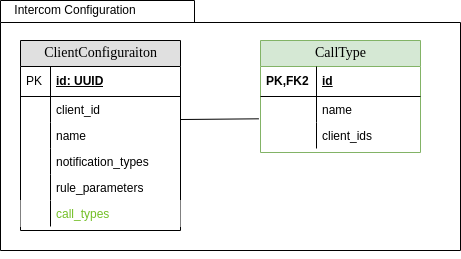
\includegraphics[width=\textwidth]{/home/joshua/FHNW/dev/IP6/IP6_Bachelorarbeit_Bericht_Cloudbasiertes_Praxisrufsystem/src/graphics/diagramms/erd_intercom_v02.drawio}
        \caption{ERD Ausschnitt - Konfiguration Gegensprechanalge}
    \end{minipage}
\end{figure}

Das Admin UI wird mit Ansichten erweitert, um CallTypes zu erstellen, anzeigen, bearbeiten und löschen.
Gleichzeitig wird der Cloudservice um Rest Endpunkte für das Lesen, Erstellen, Aktualisieren und Löschen von CallTypes erweitert.

Die Ansichten für ClientConfigurations im Admin UI werden so erweitert, dass CallTypes darauf angezeigt, hinzugefügt und entferntw erden können.
Die bestehenden Endpunkte für ClientConfiguration werden entsprechend erweitert.

\clearpage

\subsubsection{Signaling Server}

Mit WebRTC werden Peer To Peer Sprachverbindungen aufgebaut.\footnote{citation}
Bevor die Verbindung aufgebaut ist, kennen die beiden Clients sich gegenseitig noch nicht.
Die beteiligten Clients müssen Signale austauschen können um sich auf die Details der Verbindung zu einigen.
Es braucht deshalb eine Instanz, welche beide Seiten kennt und Vermittlung von Signalmeldungen übernimmt.
In Praxisruf übernimmt der Cloudservice die Funktion, Benachrichtigungen zu vermitteln.

Prinzipiell ist es möglich, den Signalaustausch in dieses Modul zu integrieren.
Dieser Ansatz hat aber zwei grosse Probleme.
Erstens ist die Grösse von Medlungen, welche über den gewählten Messaging Service (Firebase Cloud Messaging) ausgetauscht werden können beschränkt.
Meldungen zum Aufbau von WebRTC Verbindungen können diese Grösse überschreiten.\footnote{cite}
Zweitens geschieht das Versenden von Benachrichtigungen über einen asynchronen Mechanismus.
Die Signale für Sprachverbindungen sollen aber synchron ausgetauscht werden.
Es soll unmittelbar beim Versuch des Verbindungsaufbau klar sein, ob die Verbindung etabliert werden kann oder nicht.

Mit diesem Projekt wird der Cloudservice deshalb um ein weiteres Modul ''Signaling'' erweitert, welches den austausch von Signalen zwischen Clients ermöglicht.
Gleich wie das Modul für Sprachsynthese wird er unabhängig von den anderen Domänenmodulen im Cloudservice implementiert.
Alle Informationen, welche aus anderen Domänen benötigt werden, werden über Rest-Schnittstellen bezogen.
Das Modul Signaling übernimmt drittens Aufgaben.
Erstens muss es den Clients die Möglichkeit bieten, sich für Sprachverbindungen zu registrieren und diese Registrierungen verwalten.
Zweitens muss es Signalmeldungen empfangen und an die relevanten Empfänger zustellen.
Drittens muss es wann immer möglich Clients über nicht zustellbare Signale benachrichtigen.
Diese drei Funktionen müssen unabhängig von der gewählten Technologie für den Signalaustausch unterstützt werden.
Es wird ein entsprechendes Interface spezifiziert\footnote{Siehe Listing 6}.
Dieses definiert die Methoden afterConnectionEstablished und afterConnectionClosed.
Die beiden Methoden werden aufgerufen, wenn eine Verbindung geöffnet resp. geschlossen wurde.
Geöffnete Verbindungen werden in Memory geführt.
Dabei wird jede Verbindung durch eine UUID identifiziert.
Diese UUID entspricht der technischen Identifikation des entsprechenden Mobile Clients und muss, wenn sich der Mobile Client für eine Verbindung registriert mitgesendet werden.
Ein Mobile Client ist für den Signalaustausch verfügbar, wenn das Signaling Modul eine Verbindung mit seiner technischen Id kennt.
Sobald eine Verbindung geschlossen wurde, wird sie aus der Liste der in Memory Verbindungen wieder gelöscht.
Der entsprechende Mobile Client steht damit nicht mehr für den Signalaustausch zu Verfügung.

Für das Zustellen von Signalen wird die Methode sendMessage definiert.
Jede Message beinhaltet eine Payload und die Identifikation des Empfängers.
Der Signaling Service durchsucht die bekannten Verbindungen und findet die Verbindung für die Identifikation des Empfängers.
Anschliessend sendet er das Signal über die Verbindung dieses Empfängers.

Für die Verwaltung von bestehenden Verbindungen wird die Komponente ConnectionRegistry implementiert.
Diese muss Verbindungen anhand einer id registrieren und Verbindungen wieder entfernen können.
Weiter müssen Verbindungen anhand ihrer id gefunden werden können.
Die ConnectionRegistry wird als Wrapper um eine Java HashMap implementiert.
Durch die Verwendung der Map über einen Wrapper bleibt die Implementation aber unabhängig davon und kann leicht ausgetauscht werden. \footnote{Siehe Listing 7}

\clearpage

TODO: Replace with class diagram

\lstinputlisting[caption=ClientConnector.java,language=java,label={lst:ClientConnector.java}]{listings/ClientConnector.java}

\lstinputlisting[caption=ClientConnector.java,language=java,label={lst:ClientConnector.java}]{listings/ConnectionRegistry.java}

\clearpage

Die Schnittestelle des Signaling Servers nach aussen wird mit Websockets umgesetzt.
Wie die restlichen Module des Cloudservices wird auch der Singaling Server als Spring Boot Modul umgesetzt.
Mit dem Projekt Spring-Boot-Starter-Websocket, können Websocketanbindungen in einer Spring Boot Applikation umgesetzt werden.\footnote{cite}
Es wird ein WebsocketHandler implementiert, welcher unter dem Pfad ''server-url/signaling'' erreichbar ist.
Die Implementation der Websocketschnittstelle implementiert das oben beschriebene ClientConnector Interface mit der entsprechenden Funktion.

Etablierte Verbindungen müssen eindeutig einem Client zugeordnet werden können.
Diese Client Identifikation wird als Query Parameter bei Verbindungsaufbau mitgegeben und im WebsocketHandler ausgelesen.
Anschliessend wird die WebsocketSession zusammen mit der Client Identifikation in der ConnectionRegistry gespeichert.
Wird die WebsocketSession geschlossen, wird sie durch den WebsocketHandler wieder von aus der ConnectionRegistry entfernt.

Der Zugriff auf den Signaling Service darf nur für Berechtigte möglich sein.
Um dies sicherzustellen, wird der Verbindungsaufbau nur erlaubt, wenn die Anfrage dazu authentisiert ist.
Für die Authentisierung wird derselbe Meachnismus wie für Http Anfragen in den anderen Cloudservice Domänen verwendet werden.
Über die SecurityConfig des Cloudservices wird die Authentification aller Http Requests überprüft.
Diese Konfiguration sorgt dafür, das unauthentifizierte Http Requests eine entsprechende Response erhalten.
Sie verhindert allerdings nicht, dass eine Websocketverbindung aufgebaut wurde, obwohl der Request nicht authentifiziert werden konnte.
Um dies zu verhindern, muss der Http Request für den Aufbau einer Websocketverbindung notwendig sind abgefangen werden und geprüft werden, ob der Request authentifiziert wurde.\cite{cite}
Spring bietet dazu die Klasse HttpSessionHandshakeInterceptor.
Mit der Methode beforeHandshake kann der Request vor dem Verbindungsaufbau abgefangen werden und die Authentisierung überprüft werden.
Ist diese gültig, wird die Verbindung aufgebaut.
Andernfalls wird der Verbindungsaufbau abgebrochen und eine Reponse mit HttpStatue ''unauthorized'' zurückgesendet.

\clearpage

\subsubsection{Anmeldung und Registrierung}

Der Ablauf von Anmeldung und Registrierung funktioniert mit dem neuen nativen Mobile Client grundsätzlich gleich wie zuvor.
Praxismitarbeitende öffnen die Applikation und geben ihr Benutzername und Passwort ein.
Der Mobile Client verwendet diese um sich über Basic Authentication beim Cloudservice anzumelden.
Als Antowrt auf die Anmeldung gibt der Cloudservice ein JWT Token zurück.
Dieses wird für die Authentifizierung aller weiteren Anfragen an den Cloudservice verwendet.
Nachdem die Anmeldung erfolgt ist, wird eine Liste aller Clientconfigurations die dem aktuellen Benutzer zur Verfügung stehen beim Cloudservice angefragt.
Der Benutzer wählt die gewünschte Konfiguration aus und bestätigt.

\begin{figure}[h]
    \centering
    \begin{minipage}[b]{0.9\textwidth}
        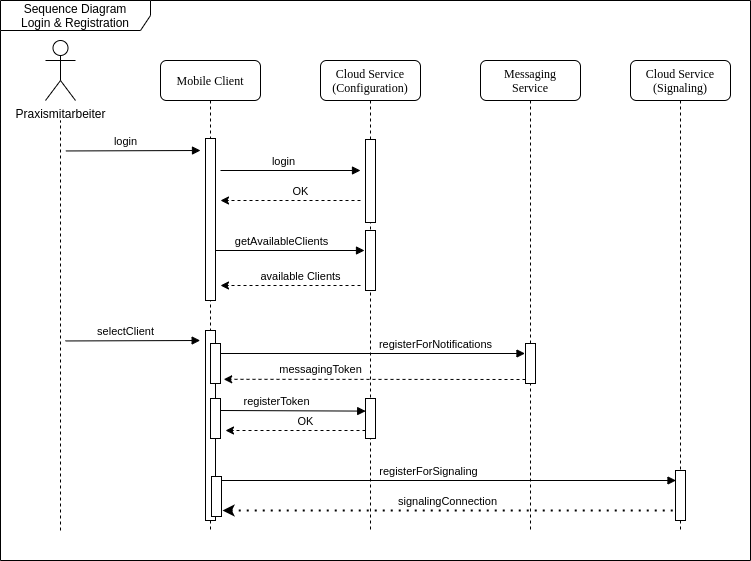
\includegraphics[width=\textwidth]{/home/joshua/FHNW/dev/IP6/IP6_Bachelorarbeit_Bericht_Cloudbasiertes_Praxisrufsystem/src/graphics/diagramms/Sequence_Registration}
        \caption{Mockup Home}
    \end{minipage}
\end{figure}

Danach wird diese Konfiguration geladen und die Hauptansicht angezeigt.
Die geladene Konfiguration beinhaltet alle Informationen die nötig sind um Buttons für Benachrichtigungen und Sprachverbindungen anzuzeigen.
Im Hintergrund muss sich der Mobile Client nun für Benachrichtigungen und Sprachverbindungen registrieren.
Für Benachrichtigungen registriert er sich zuerst beim Messaging Service.
Er erhält ein Token, welches den Client beim Messaging Service identifiziert.
Dieses Token sendet der Mobile Client zusammen mit der gewählten Konfiguration an den Cloudservice.
Dieser persistiert die Registrierung bei sich und kann sie verwenden um Benachrichtigungen an diesen Client zuzustellen.
Für Sprachverbindungen muss zudem eine Verbindung zum Signlaing Modul des Cloudservices aufgebaut werden.
Dazu wird wie in Kapitel 5.4.5 beschrieben eine Websocketverbindung geöffnet.

\clearpage
\subsubsection{Signalmeldungen}

Dieses Kapitel beschreibt die Signalmeldungen, welche für Sprachverbindungen verwendet werden.

\begin{figure}[h]
    \centering
    \begin{minipage}[b]{0.4\textwidth}
        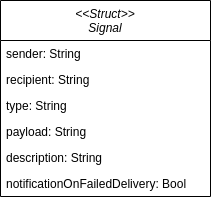
\includegraphics[width=\textwidth]{graphics/diagramms/Class_Signal_V01}
        \caption{Signal (Mobile Client)}
    \end{minipage}
\end{figure}

Alle Signalmeldungen beinhalten Identifikation von Sender und Empfänger.
Diese werden vom Signalingserver verwendet, um die Signale korrekt weiterzuleiten.
Type, Payload und Description werden im Mobile Client verwendet, um das Signal korrekt zu verarbeiten und Verbindungen aufzubauen.
Das Flag notificationOnFailedDelivery wird im Cloudservice ausgewertet.
Wenn ein Signal nicht zugestellt werden kann und dieses Flag TRUE ist, wird der Empfänger mit einer asynchrone Benachrichtigung darüber informiert.
Dazu wird das bestehende Notification Modul des Cloudservices verwendet.
Für die Verwaltung von Sprachverbindungen werden insgesamt sechs Typen von Signalmeldungen definiert.

OFFER: Ein Offer wird vom Initiator der Sprachverbindung an die Empfänger gesendet.
Es beinhaltet die SDP\footnote{Sesseion Description Protocol} Informationen des Initiators.  \\

ANSWER: Eine Answer wird vom Empfänger eines Offers an den Initiator der Sprachverbindung gesendet.
Es beinhaltet SDP\footnote{Sesseion Description Protocol} Informationen des Empfängers.

ICE CANDIDATE: Ein RTCIceCandidate beschreibt Routing- und Protokollinformationen, die für den Verbindungsaufbau verwendet werden.
Nach Verarbeitung von OFFER und ANSWER tauschen Initiator und Empfänger solange ICE CANDIATE Signale aus, bis sie sich auf einen Kandidaten geeinigt haben.\\

END: Wird von Empfänger oder Initiator versendet, nachdem die Verbindung durch tippen des Auflegen-Button in der Applikation beendet wurde.
Empfang dieses Signal führt dazu, dass alle offene Sprachverbindungen beendet werden.\\

UNVAILABLE: Wenn der Signalinvserver ein Signal nicht zustellen kann, wird das Ziel wenn möglich über eine Benachrichtigung informiert.
Zudem wird ein Unavailable Signal zurück an den Sender gesendet.
So weiss dieser, dass der gewünschte gesprächspartner nicht verfügbar ist. \\

DECLINE: Praxismitarbeitende haben die Möglichkeit den Empfang von Anrufen zu deaktivieren.
Wird ein Signal empfangen während Anrufe deaktiviert sind, sender der Mobile Client ein DECLINE Signal zurück. \\

\clearpage

Praxismitarbeitende können Sprachverbindungen zu anderen Clients aufbauen indem sie auf den entsprechenden Button in der Praxisruf App tippen.
Zum Zeitpunkt an dem der Button getippt wird, weiss der Mobile Client noch nicht, zu welchen Clients diese Verbindung aufgebaut werden soll.
Als erstes muss deshalb beim Cloudservice angefragt werden, welche Clients mit dem betätigten Button angesprochen werden sollen.
Der Cloudservice bietet dazu einen Endpoint an über den der vollständige CallType des verwendeten Buttons hinterlegt sind geladen werden können.
Nachdem diese Informationen geladen sind, können Sprachverbindungen zu allen relevanten Clients aufgebaut werden.
Dazu müssen mehrere Signalmeldungen ausgetauscht werden.
Der auslösende Client initialisiert die Peer to Peer Verbindung auf seiner Seite und sendet für jeden Gesprächspartner ein Angebot (OFFER), welches signalisiert, dass er eine Sprachverbindung aufbauen möchte.
Der Cloudservice findet die Verbindung des relevanten Empfängers und leitet das Signal über diese Verbindung weiter.
Der Empfänger nimmt das Angebot (OFFER) entgegen, initialisiert die Verbindung auf seiner Seite und sendet eine Antwort (ANSWER).
Diese wird wiederum über den Cloudservice weitergeleitet.
Der auslösende Client empfängt die Antwort (ANSWER) und ergänzt die notwendigen Verbindungsinformationen.

Folgende Graphik zeigt den initialen Ablauf des Verbindungsaufbau:

\begin{figure}[h]
    \centering
    \begin{minipage}[b]{0.9\textwidth}
        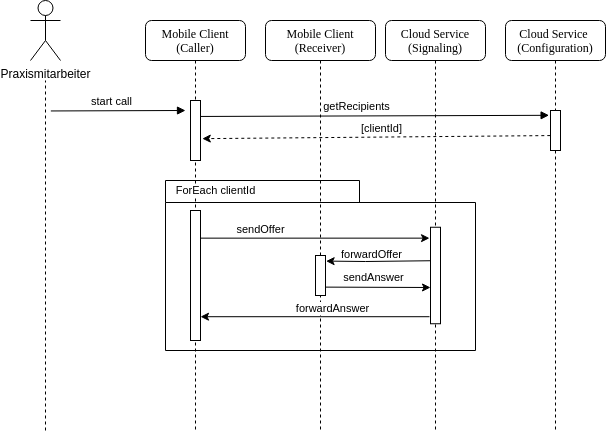
\includegraphics[width=\textwidth]{graphics/diagramms/Sequence_Intercom_Broking_V02}
        \caption{Ablauf Verbindungsaufbau Gegensprechanalge}
    \end{minipage}
\end{figure}









Der Mobile Client kennt nun die technischen Identifikatoren der Clients, zu denen eine Verbindung aufgebaut werden soll.
Um die Peer To Peer Verbindung zu diesen Clients aufzubauen, müssen nun weitere Nachrichten mit dem Cloudservice ausgetauscht werden.
Alle verfügbaren Clients haben sich bei der Anmeldung mit dem Cloudservice verbunden.
Der Cloudservice führt eine Liste über die verfügbaren Verbindungen und die dazugehörigen technischen Identifikatoren.
Über diese Verbindungen werden nun die Nachrichten ausgetauscht die zum aufbauen der WebRTC Verbindung benötigt werden.
Der Austausch dieser Nachrichten folgt dem Interactive Connection Establishment Protokoll (ICE).
Der Client initialisiert für jede der erhaltenen client Ids einen Rtc Connection.
Dies dient als Endpunkt der Connection auf seiner Seite.
Anschliessend Sendet der Client ein Anfrage an den Cloudservice.
Dieses Anfrage beinhaltet das ICE Offer und die Client Ids des von Ausgangs- und Ziel-Client.
Der Cloudservice findet die Verbindung des Zieles anhand der Client Id und leitet das ICE Offer und Ausgangs Client Id über die registrierte Verbindung an den Empfänger weiter.
Wenn der Empfänger das ICE Offer erhält, initialisiert er auf seiner Seite die Rtc Connection und sendet eine Anfrage mit ICE Antwort und originaler Ausgangs Client Id an den Server zurück.
Dieser leitet die Anfrage dann analog dem ICE Offer an die Verbindung des ausgehenden Clients weiter.
Sobald dieser die Antwort erhält, ist die Rtc Connection bestätigt und die Sprachverbindung ist initialisiert.

\clearpage


\subsubsection{Anbindung Mobile Client an Singaling Server}

Für den Aufbau von Sprachverbindungen zwischen Mobile Clients müssen mehrere Signalmeldungen ausgetauscht werden.
Der Cloud Service wird im Rahmen dieses Projektes um eine Websocket Schnittstelle erweitert, welche dies ermöglicht.\footnote{Vgl. Kapitel 5.4}
Als Technologie für diese Schnittstelle werden Websockets verwendet.
Der Api Service wird dementsprechend erweitert, um Websocket Verbindungen zu ermöglichen.
Dies beinhaltet den Auf- und Abbau von Websocket Verbindungen, sowie das Senden und Empfangen von Meldungen über diese Verbindung.
Weiter muss die Verbindung konstant offen gehalten und im Fehlerfall erneut aufgebaut werden können.

Der Austausch von Signalmeldungen ist der einzige Anwendungsfall in Praxisruf, der Websocketverbindungen benötigt.
Deshalb wird auf eine generische Integration von Verbindungen analog von Http Verbindungen\footnote{Vgl. Kapitel 5.2.2} verzichtet.
Stattdessen wird eine Extension Klasse PraxisrufApi+Signaling nach folgendem Muster erstellt:

\lstinputlisting[caption=PraxisrufApi+Signaling.swift,language=java,label={lst:PraxisrufApi+Signaling.swift}]{listings/PraxisrufApi+Signaling.swift}

Die Signaling Extension kann immer genau eine offene Verbindung verwalten.
Diese wird als Instanzvariable innerhalb des Services geführt.
Der Status dieser Verbindung kann als Computed Property "disconnected" intern abgefragt werden.
Die Extension bietet Methoden um den Signaling Service zu Verbinden.
Eine Verbindung wird dabei immer spezifisch für die aktuell gewählte Client Configuration geöffnet. \footnote{Vgl. Kapitel X.X}
Weiter werden Methoden angeboten, um Pingsignale zu senden oder die Verbindung zu trennen.
Zudem bietet die Extension Methoden, um Signalmeldungen über die geöffnete Verbindung zu senden,
sowie eine Methode um empfangene Signalmeldungen zu verarbeiten.

Für die Integration der Singalingverbindung in den Rest der Applikation, wird das Protokoll PraxisrufApiSignalingDelegate definiert.

\lstinputlisting[caption=PraxisrufApiSignalingDelegate.swift,language=java,label={lst:PraxisrufApiSignalingDelegate.swift}]{listings/PraxisrufApiSignalingDelegate.swift}

Vor dem Versenden einer Signal- oder Pingmeldung wird überprüft, ob eine Verbindung geöffnet und Fehlerfrei ist.
Ist dies nicht der Fall, wird die Verarbeitung die onConnectionLostMethode des Delegates aufgerufen.
Die Implementation dieses Delegates ist dafür verantwortlich, die Verbindung wieder zu öffnen.
Die Methoden onSignalReceived resp. onErrorReceived werden aufgerufen wenn ein Signal resp. eine Fehlermeldung empfangen wurde.
Im Fehlerfall soll wenn nötig eine Fehlermeldung angezeigt werden und die Verbindung repariert werden.
Wenn eine Signalmeldung empfangen wurde, muss diese an die Applikation zu Verarbeitung weitergereicht werden.

\clearpage

\subsubsection{Signalverarbeitung im Mobile Client}

Neben austausch von Signalen muss auch die Sprachverbindung selbst verwaltet werden.
Die Details der Sprachverbindung sind vendor spezifisch.
Es wird deshalb eine eigene Klasse CallClient erstellt.
Diese ist für das Verwalten von Verbindungen verantwortlich.
Bei eingehenden Verbindungen muss sie signale empfangen, die Verbindung erstellen.
Wenn nötig Antowrt Signale erstellen und zurückgeben.
Bei ausgehenden Verbindungen muss sie Verbindung initialisieren.
Es muss Signal erstellt und versendet werden.
Weiter müssen Methoden angeboten werden um die Unterhaltung oder das Microphon zu muten.
Und um die Verbindung zu schliessen.
Und um den bei Änderung des internen Status, das UI entsprechend zu aktualisieren.

Um die Integration der Sprachverbindung möglichst unabhängig und auswechselbar zu machen, wird der CalLClient nicht direkt in der View verwendet.
Stattdessen definiert der CallClient ein Delegate Protocol, welches die notwendigen Callbacks definiert.

\lstinputlisting[caption=CallClientDelegate.swift,language=java,label={lst:CallClientDelegate.swift}]{listings/CallClientDelegate.swift}

Um Anrufe in der Applikation verwenden zu können müssen CallClient und PraxisrufApi+Signaling in die Benutzeroberfläche integriert werden.
Beide Applikationen definieren ein Delegate Protocol, welches die Funktionen spezifiziert, über welche die Komponenten eingebunden werden können.
Es wird eine weitere Serviceklasse mit dem Namen CallService implementiert, welche beide Delegate Protocols implementiert.
Dieser Service instanziert CallClient und PraxisrufApi+Signaling und registriert sich anschliessend als Delegate bei beiden Instanzen.
Der CallService selbst wird in der View verwendet.
Er nimmt Benutzereingaben entgegen und delegiert die entsprechende Funktionalität an den CallClient und SignalingClient.

Wenn der Benutzer einen Anruf startet, wird die View für aktive Anrufe geladen.
Diese initialisiert den Anruf über den CallService.
Der CallService ruft dazu als erstes den CallClient auf.
Der CallClient initialisiert die lokalen Verbindungsinformationen und erstellt ein Signel, um den Empfänger zu informieren.
Dieses Signal gibt er an den CallService weiter.
Der CallService leitet das Signal an den SignalingClient weiter, welcher das Versenden an den Cloud Service übernimmt.

\clearpage
\begin{figure}[h]
    \centering
    \begin{minipage}[b]{0.8\textwidth}
        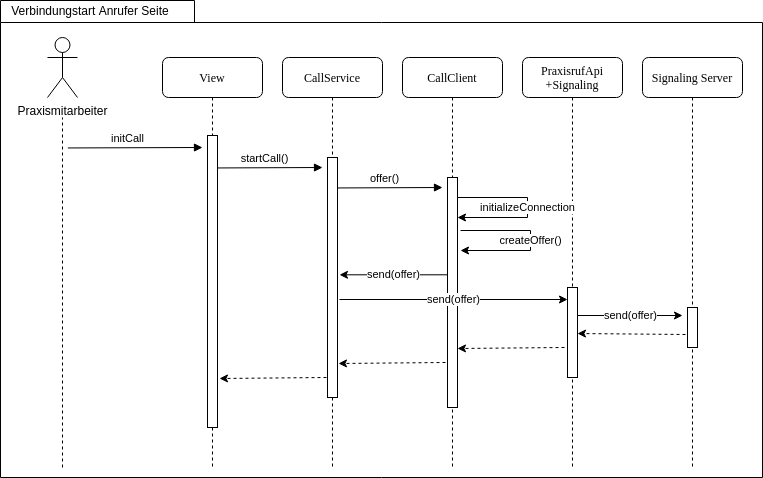
\includegraphics[width=\textwidth]{/home/joshua/FHNW/dev/IP6/IP6_Bachelorarbeit_Bericht_Cloudbasiertes_Praxisrufsystem/src/graphics/diagramms/Sequence_MobileClient_Caller_Signaling.drawio}
        \caption{MobileClient - Anruf Starten Signal}
    \end{minipage}
\end{figure}

Das versendete Signal wird über das Signaling Modul des Cloud Service an den Empfänger übermittelt.
Dieser empfängt das Signal über den SingalingClient.
Der SignalingClient gibt das Signal über onSignalReceived an den CallService weiter.
Der CallService aktiviert die Ansicht für aktive Anrufe und leitet das Signal an den CallClient weiter.
Der CallClient initialisiert die lokalen Verbindungsinformationen und erstellt eine Signal zur Bestätigung.
Dieses Signal wird wiederun über den CallService zum SignalingClient weiter zum Cloud Service versendet.
Auf Starterseite, kann diese Bestätigung weiterverarbeitet werden.

\begin{figure}[h]
    \centering
    \begin{minipage}[b]{0.8\textwidth}
        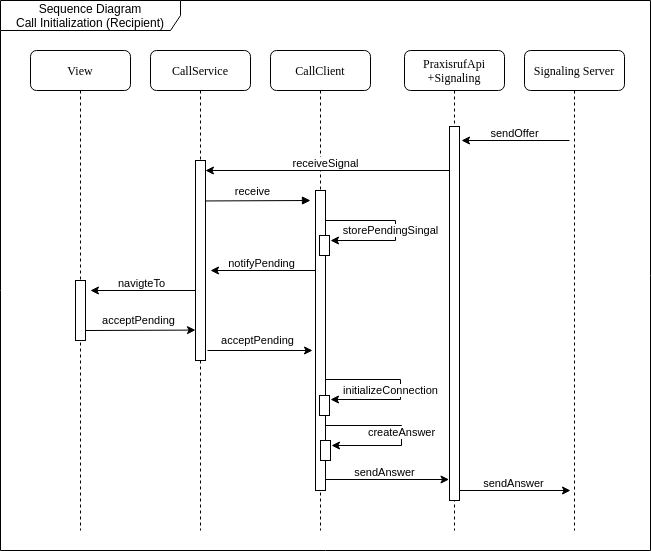
\includegraphics[width=\textwidth]{/home/joshua/FHNW/dev/IP6/IP6_Bachelorarbeit_Bericht_Cloudbasiertes_Praxisrufsystem/src/graphics/diagramms/Sequence_MobileClient_Receiver_Signaling.drawio}
        \caption{Mobile Client Anruf Empfangen Signal}
    \end{minipage}
\end{figure}

\clearpage

\subsubsection{Integration WebRTC in Mobile Client}

Gekapselt im Service CallClient.
Managed den State von Sprachverbindungen.
Kommuniziert nur über den Delegate mit dem Rest der Applikation.
Verwendet die Klassen der WebRTC iOS Library um Peer To Peer Verbindungen zu machen.
Die dazu notwendigen Signale werden über Delegate / Signaling Server ausgetauscht.

\subsubsection{Verpasste und vergangene Anrufe}

Verpasste geben Push Benachrichtigung
Verpasste müssen quittiert werden.
Vergangene erscheinen in Inbox.
Vergangene müssen nicht quittiert werden.

\subsubsection{Unterhaltung}

Mute Button
Audio Off Button
End Call Button


\subsubsection{Verbindungsende}

Button antippen

\clearpage
